\documentclass[12pt]{article}
\usepackage{amsmath,amsthm,amssymb}
\usepackage{graphicx}
\usepackage{cite}
\pagestyle{myheadings}
\author{Joseph McDonald}

\textwidth=7in
\textheight= 9in

\topmargin=-0.5in
\oddsidemargin=-0.25in

\newcommand{\xbar}{\bar{x}}
\newcommand{\V}[1]{\boldsymbol{#1}}
\newcommand{\E}[0]{\mathbb{E}}
\title{Parallelizing AdaBoost and Decision Trees}

\begin{document}

%\begin{abstract}
%I present a parallelized construction of decision trees to be used in AdaBoost
%\end{abstract}

\maketitle

\section{Introduction}
Binary and multiclass classification is a fundamental problem in machine learning and is commonly one of the first concepts to be studied in an introductory course. In the context of binary classification, a labeled observation is a coordinate pair $(x, y)$ where $x\in\mathbb{R}^d$ is a vector of data associated with the observation (feature vector) and $y\in\{1, -1\}$ is the corresponding label of the observation. For example, $x_i$ might be a point in $\mathbb{R}^2$ representing the height and weight of the $i$th individual in a data set while the value of $y_i$ may correspond to the person's gender. The goal in classification is to accurately predict the label of a given observation using its feature vector. In this setting, the scenario of supervised learning involves using a training set of labeled observations $(x_i, y_i)$ to construct a prediction function $h$, one that takes a feature vector $\hat{x}$ and gives a prediction on the corresponding label $h(\hat{x})=\hat{y}$. It is common to use a separate set of test data to check the accuracy of the predictor, data that hasn't been used for training. There are many methods used to obtain a predictor for classification in supervised learning, and the class of ensemble methods concerns combining several predictors to obtain one.

Suppose now there exists an algorithm that, for any set of training data, is guaranteed to give you a predictor that has at least 50\% accuracy. Such an algorithm is called a weak learning algorithm since it yields a predictor that performs marginally better than guessing randomly. These prediction functions that a weak learning algorithm returns are called base classifiers, and a natural question arises about whether we can use a combination of weak learners to get a stronger one with much better accuracy and what this sort of ensemble method would look like. Ensemble methods like this are called boosting, and the algorithm AdaBoost introduced in \cite{no1} accomplishes this through successive rounds of training a weak learner to the data and subsequently re-weighting the training samples \cite{no1}.

The goal of this project is to implement a parallelized version of a commonly used weak learner, decision trees, to improve the running time of AdaBoost. We give a short overview of AdaBoost and decision trees in the next section, describe the implementation of the decision trees, the data sets used and the results t 

\section{AdaBoost}
The beauty of AdaBoost is in using a relatively inaccurate weak learning algorithm to produce a much more accurate prediction function. As mentioned, in each iteration of AdaBoost the weak learner selects a base classifier $h: \mathbb{R}^n\rightarrow\{1,-1\}$ from a set of functions $H$. The weak learner chooses in particular the base classifier  We give the algorithm below.\\
\\
{\sc AdaBoost}: $S = \{(x_i,y_i):i = 1\ldots n\}$
\begin{enumerate}
\itemsep1pt \parskip0pt \parsep0pt
\item {\bf for $i=1$ to $n$}
\item \quad $D_1(i) = \frac{1}{n}$
\item {\bf for $t=1$ to $T$}
\item \quad $h_t$ = {\sc WeakLearner}$(S\sim D_t)$ with weighted error $\epsilon_t$
\item \quad $\alpha_t = \frac{1}{2}\log(\frac{1-\epsilon_t}{\epsilon_t})$
\item \quad $Z_t = 2[\epsilon_t(1-\epsilon_t)]^{1/2}$ (normalization factor)
\item \quad {\bf for $i = 1$ to $n$}
\item \quad \quad $D_{t+1}(i) = \frac{D_t(i)\exp(-\alpha_t y_i h_t(x_i))}{Z_t}$
\item $g = \sum_{t=1}{T} \alpha_t h_t$
\item {\bf return} $\mbox{sign}(g)$
\end{enumerate}



\section{Decision Trees}
Decision trees are a well-known method useful for classification which partitions the feature space into rectangular regions and gives each region the most common label among the training set points it contains. Each partition of the feature space is made along coordinate axes and done in a heirarchical way. Starting with the entire space, a line parallel to an axis divides it into two regions and then the same is done for these resulting regions. This process is repeated many times until the space is partitioned into several rectangles, like the example in Figure 1 (\cite{HTF}).

\begin{figure}[b!]
\centering
\begin{minipage}{0.45\textwidth}
\centering
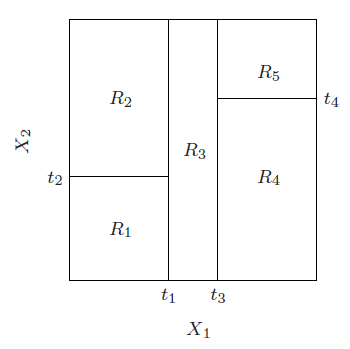
\includegraphics[width=2.5in]{partition}
\caption{space partitioned by a decision tree}
\end{minipage}\hfill
\begin{minipage}{0.45\textwidth}
\centering
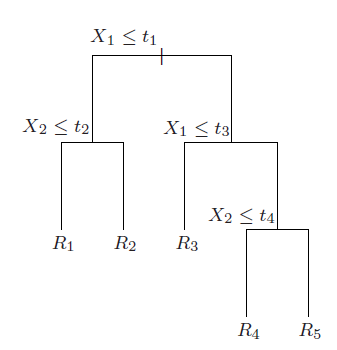
\includegraphics[width=2.5in]{dectree}
\caption{decision tree}
\end{minipage}
\end{figure}

 In that depiction, the lines drawn at $t_i$ represent the $i$th division of the space. Since each region is divided in two, this gives rise to a binary tree where each node represents a line drawn to partition the region existing before that node. The tree corresponding to Figure 1 is given in Figure 2 (\cite{HTF}). As depicted in the two figures, the splits are done in a heirarchical way that . The feature space is partitioned along coordinate axes, which gives rise to decision. The most common way to partition the feature space is along coordinate axes. 

%\maketitle
%
%\section{Introduction}
%Binary and multiclass classification is a fundamental problem in machine
%learning and is commonly one of the first concepts to be studied in an
%introductory course, the goal being to accurately predict the label of a given
%observations using the data associated with the observation. In the context of
%binary classification, a labeled observation (or sample point) is a coordinate
%pair $(x, y)$ where $x\in\mathbb{R}^d$ is a vector of data associated with the
%observation (feature vector) and $y\in\{1, -1\}$ is the corresponding label of
%the observation. This classification, and even prediction in general, commonly
%splits up into two different scenarios, supervised and unsupervised learning.
%Supervised learning involves taking a set of labeled observations (training
%set) and using it to construct a prediction function, one that can take a new
%feature vector and predict the corresponding label. There are many methods used
%for classification in supervised learning, including support vector machines,
%decision trees, online algorithms, and many others.
%
%A weak learning algorithm, or weak learner, is an algorithm that, given a set of training data, yields a predictor with performance of at least 50\% percent accuracy, or just better than random guessing. The prediction functions that a weak learner returns are called base classifiers. There was an important question asking whether the base classifiers from a weak learner could somehow be joined together to produce a strong learner, or an algorithm that gives a prediction function of arbitrary accuracy.
%
%Boosting is a category of methods that addresses this question, which Freund and Schapire
%successfully answered with their algorithm AdaBoost. AdaBoost, which stands for adaptive boosting, builds
%a more accurate predictor through successive rounds of training a weak learner
%to the data and subsequently re-weighting the training samples \cite{no1}. 




%\begin{thebibliography}
%\bibitem{FS} Yoav Freund Rob Schapire

%\bibitem{HTF} Hastie Friedman Tibshirani

%\bibitem{Mohri} Mohri

%\bibitem{no4} Wiki
%\end{thebibliography}
\end{document}



